\documentclass[a4paper,12pt]{article}
    \usepackage[utf8]{inputenc}
    \usepackage[T1]{fontenc}
    \usepackage[hungarian]{babel}
    \usepackage{graphicx}
    \usepackage{geometry}
    \geometry{a4paper,
                 tmargin = 35mm, 
                 lmargin = 25mm,
                 rmargin = 30mm,
                 bmargin = 30mm}
    \usepackage{mathtools}
    \usepackage{amsmath}
    \usepackage{color}
    \usepackage{setspace}
    \usepackage{amsmath,amssymb}
    \usepackage{float}
    \usepackage{listings}
    
    \usepackage{indentfirst}
	\usepackage{subfig}
	    
    \renewcommand\thesection{\Roman{section}.}
    \renewcommand\thesubsection{\thesection\arabic{subsection}}
    \renewcommand\thesubsubsection{}
    
\begin{document}

\linespread{1.2}

\begin{titlepage}

	\centering
	\centering
	
\includegraphics[width=0.66\textwidth]{../elte.jpg}\par\vspace{1cm}
	{\scshape\LARGE ELTE Faculty of Science\par}
	\vspace{3cm}
	{\scshape\Large Egykristály röntgendiffrakció\par}
	\vspace{1cm}
	{\large\itshape Alex Olar \par}
	\vspace{3cm}
	{\large 2018 \par}

\end{titlepage}

\onehalfspacing

\begin{abstract}
	A mérés során megismerkedtünk az egykristály röntgendiffrakcióval.
	A mérés során zafír, só és szilícium egykristályokat vizsgáltunk.
\end{abstract}

\tableofcontents

\newpage

\section{A mérés menete}

\par A méréshez a Laue-féle diffrakciós berendezést használtuk. A mérés kiértékeléséhez
az \textit{Orient Express} nevű programot használtam. Ennek bemenetén egy képet és
megfelelő egykristály rács paraméterket kellett megadni, amiket szintén megkaptunk.
A szoftver ezeke után meghatározta a megfelelő Miller-indexeket. A szoftver
segítségével ezután szimulálni lehetett a minta forgatását ami után a rácsvektorokat
be lehetett forgatni a labor rendszer irányába (amennyiben azok merőlegesek).
Error sztereogradikus leképzeséket készítettem.

\section{ Kiértékelés}

\par A képek a következő paraméterekkel készültek:

\begin{table}[H]
	\centering
	\begin{tabular}{|c||c|}  \hline
		Minta \textit{távolsága}         & 35.23 mm \\ \hline
		Imaging Plate \textit{szélesség} & 94.18 mm \\ \hline
	\end{tabular}
	\caption{Mérési elrendezés}
\end{table}

\subsection{ NaCl egykristály}

\par A konyhasóhoz kaptunk kész adatokat, melyek a lentebbi képről
leolvashatóak. A rácstávolság $5.640 A$, míg a tárgytávolság $3.0 cm$
ezekkel az adatokkal az indexelés a következőképpen néz ki:

\begin{figure}[H]
	\centering
	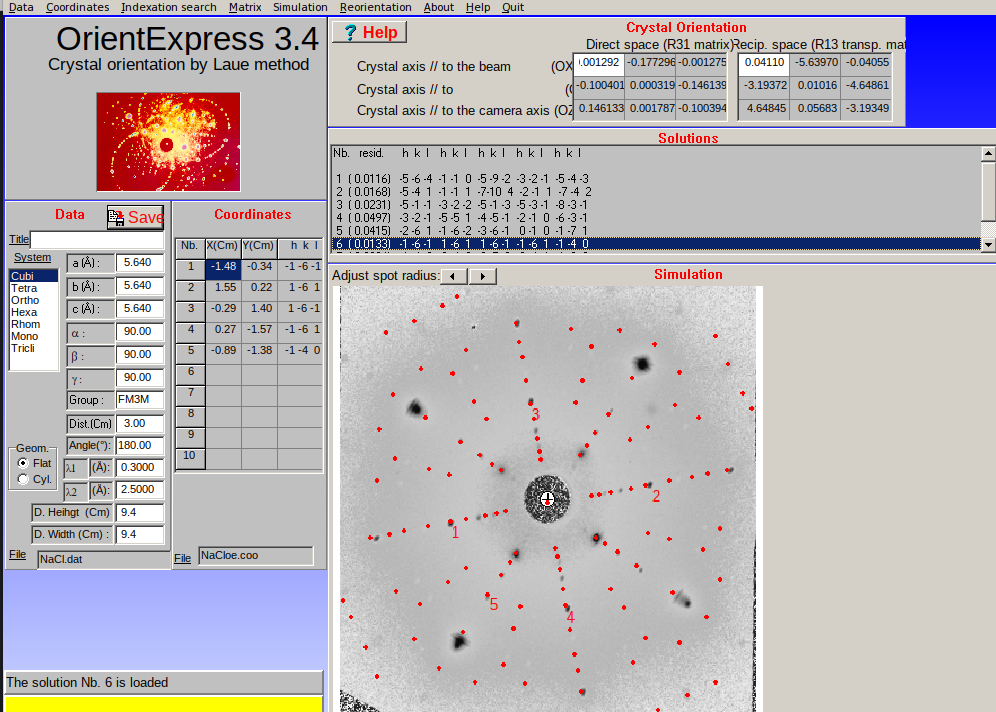
\includegraphics[width=0.6\textwidth]{NaCl-indexed-data.png}
	\caption{Adatok}
\end{figure}

\par Az indexelés adatai:

\begin{table}[H]
	\centering
	\begin{tabular}{|c|c||c|c|c|}  \hline
		x     & y     & h  & k  & l  \\ \hline
		-1.48 & -0.34 & -1 & -6 & -1 \\ \hline
		1.55  & 0.22  & 1  & -6 & 1  \\ \hline
		-0.29 & 1.40  & 1  & -6 & -1 \\ \hline
		0.27  & -1.57 & -1 & -6 & 1  \\ \hline
		-0.89 & -1.38 & -1 & -4 & 0  \\ \hline
	\end{tabular}
	\caption{A helyes indexelés eredménye}
\end{table}

\par Valamint a sztereografikus kép:

\begin{figure}[H]
	\centering
	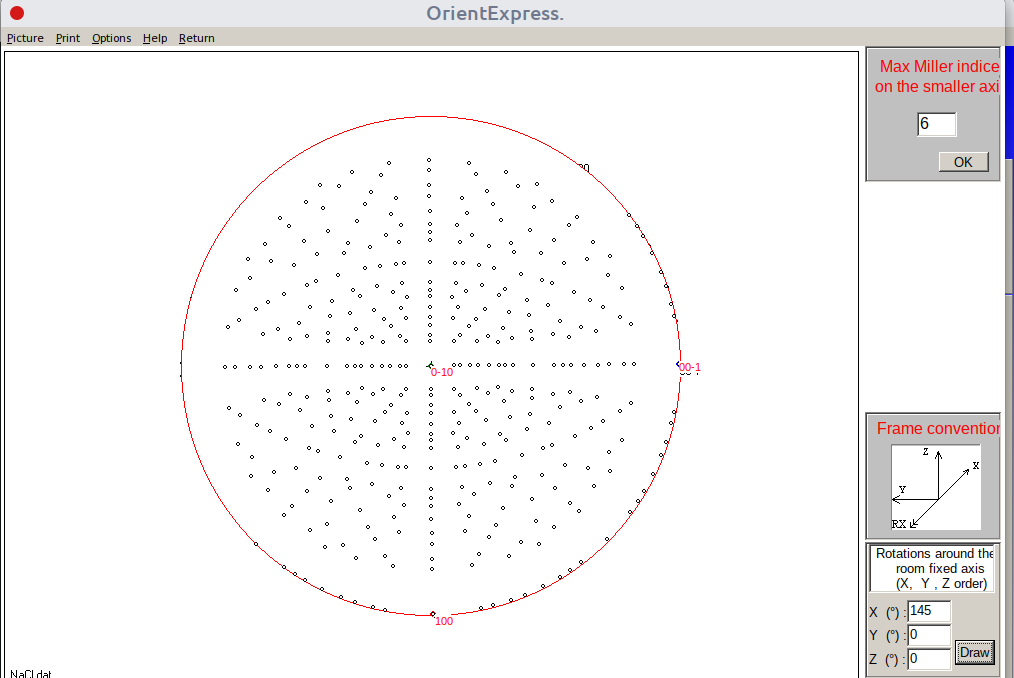
\includegraphics[width=0.6\textwidth]{NaCl-stereo.png}
	\caption{Stereo}
\end{figure}

\subsection{ Si egykristály}

\par A $Si$ már ténylegesen mértük, az adatai a lentebbi képről
leolvashatóak. A rácstávolság $5.431 A$, míg a tárgytávolság már a leírás
elején közült:

\begin{figure}[H]
	\centering
	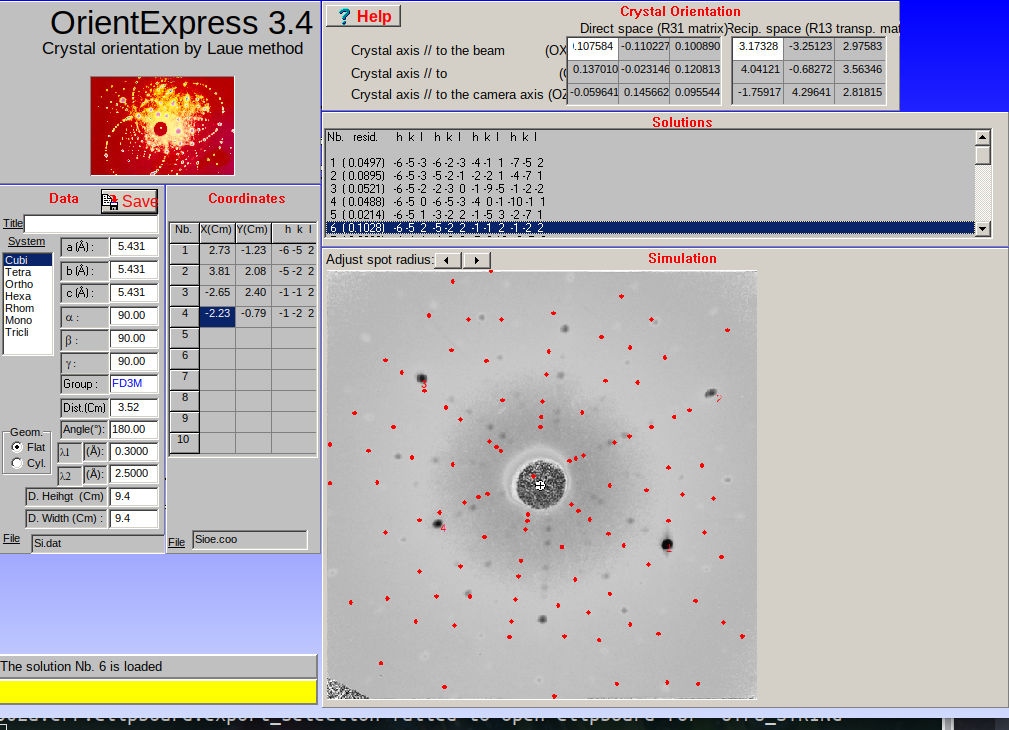
\includegraphics[width=0.6\textwidth]{./valid_indexation/Si.png}
	\caption{Adatok}
\end{figure}

\par Az indexelés adatai:

\begin{figure}[H]
	\centering
	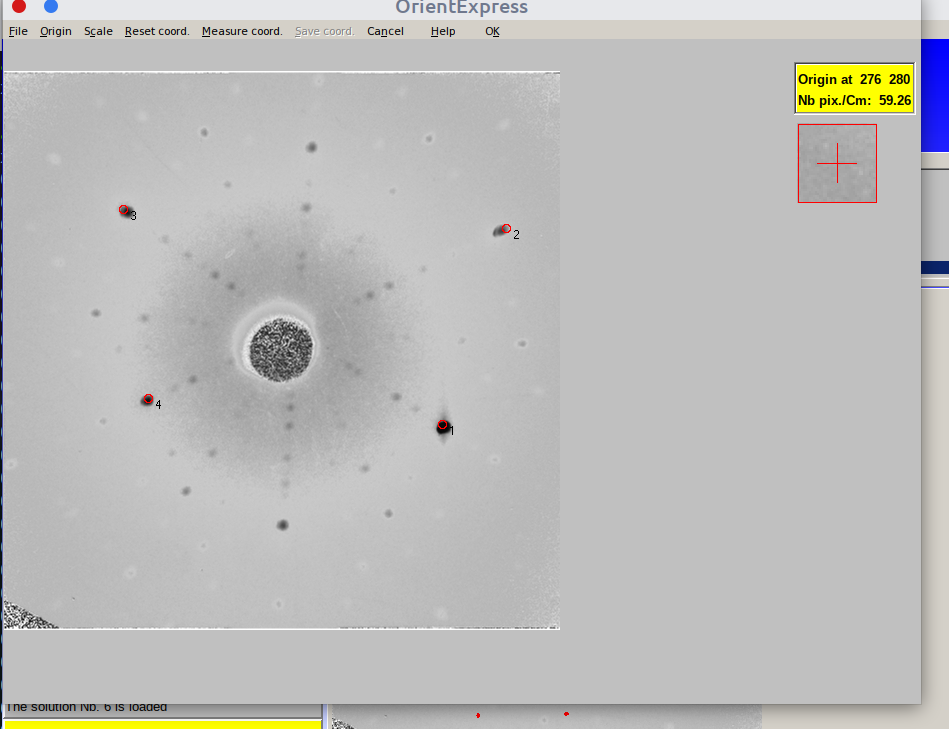
\includegraphics[width=0.6\textwidth]{./valid_indexation/Si-coords.png}
	\caption{Adatok}
\end{figure}

\begin{table}[H]
	\centering
	\begin{tabular}{|c|c||c|c|c|}  \hline
		x     & y     & h  & k  & l  \\ \hline
		2.73 & -1.23 & -6 & -5 & 2 \\ \hline
		3.81  & 2.08  & -5  & -2 & 2  \\ \hline
		-2.65 & 2.40  & -1  & -1 & 2 \\ \hline
		-2.23 & -0.79 & -1 & -2 & 2  \\ \hline
	\end{tabular}
	\caption{A helyes indexelés eredménye}
\end{table}

\par Valamint a sztereografikus kép:

\begin{figure}[H]
	\centering
	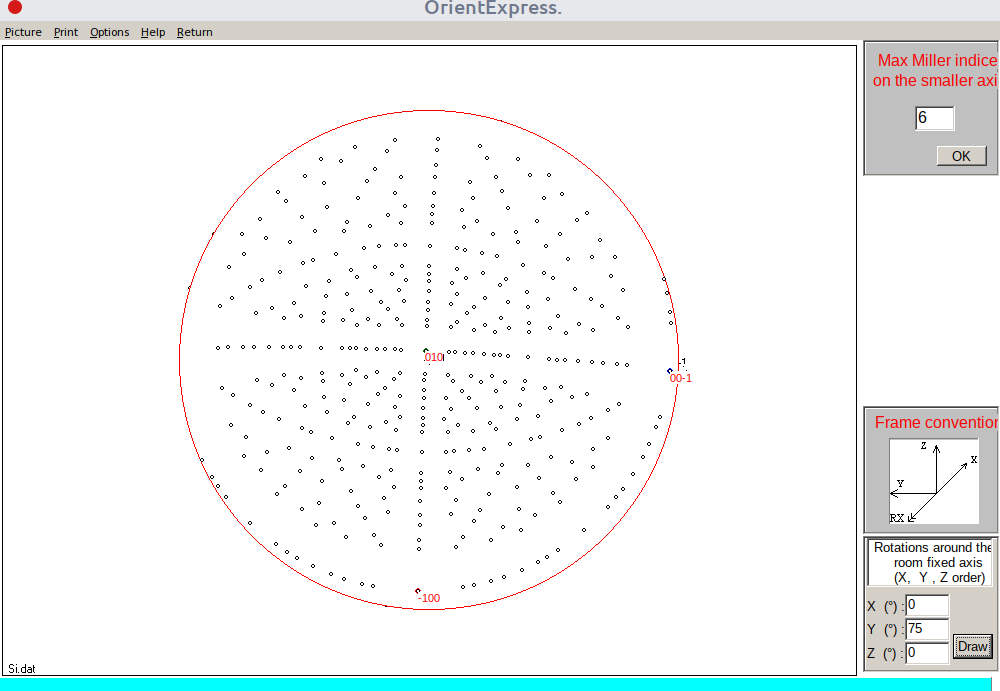
\includegraphics[width=0.6\textwidth]{./valid_indexation/Si-stereo.png}
	\caption{Stereo}
\end{figure}

\subsection{ Zafír egykristály}

\par A $Si$ már ténylegesen mértük, az adatai a lentebbi képről
leolvashatóak. A rácstávolság $5.128 A$, míg a tárgytávolság már a leírás
elején közült. Ellenben itt nem köbös rácsról van szó, így egy közelítő
rácsot használtunk, az adatokat megkaptuk természetesen.

\begin{figure}[H]
	\centering
	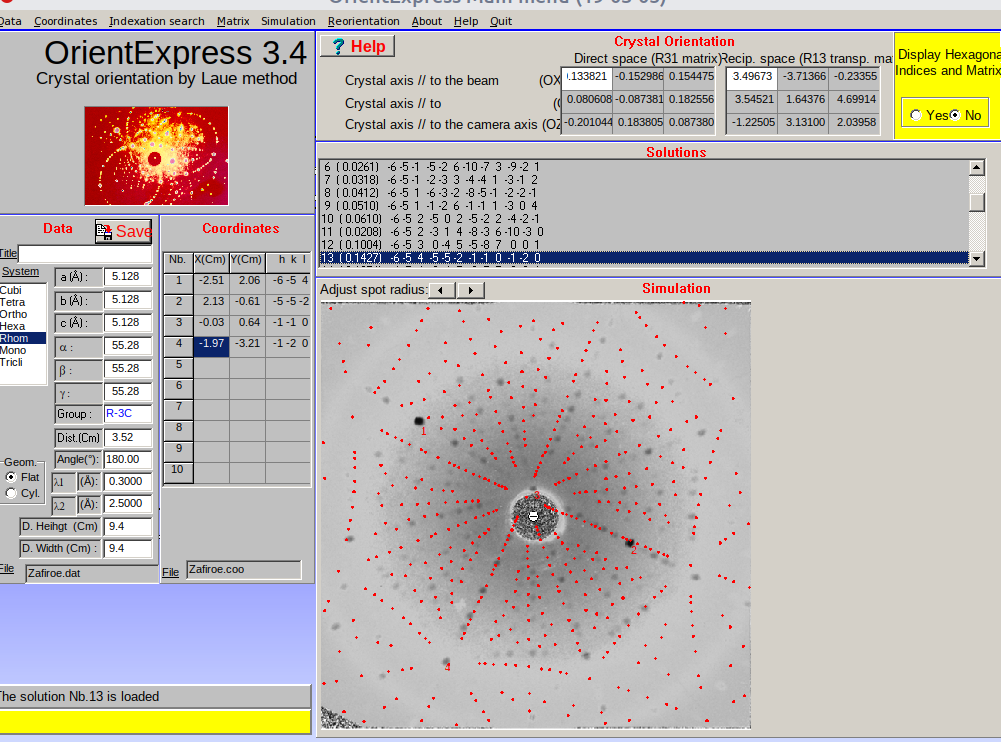
\includegraphics[width=0.6\textwidth]{./valid_indexation/Zafir.png}
	\caption{Adatok}
\end{figure}

\par Az indexelés adatai:

\begin{figure}[H]
	\centering
	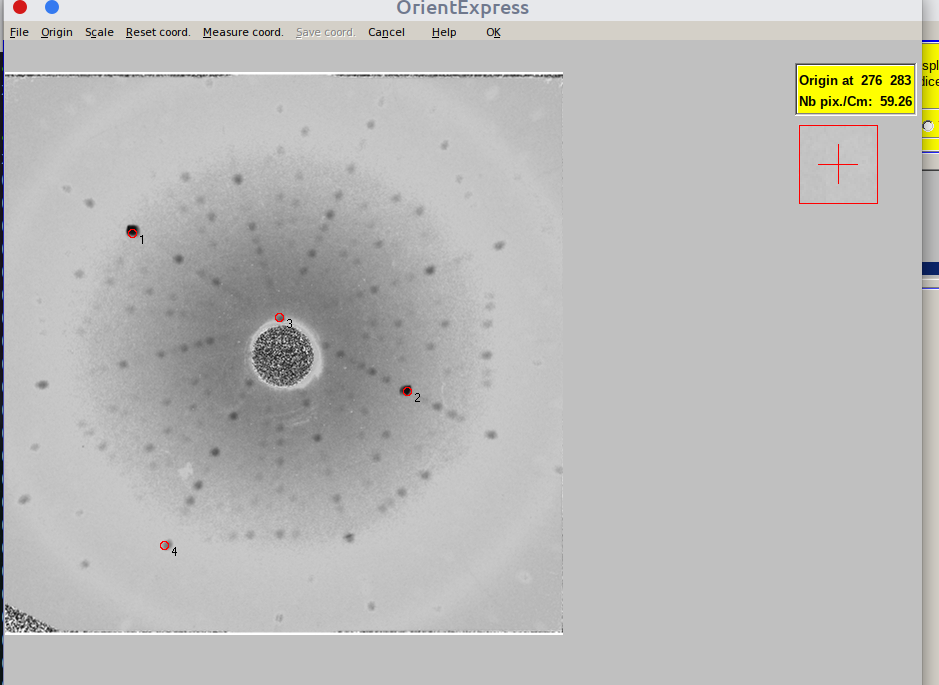
\includegraphics[width=0.6\textwidth]{./valid_indexation/zafir-coords.png}
	\caption{Adatok}
\end{figure}

\begin{table}[H]
	\centering
	\begin{tabular}{|c|c||c|c|c|}  \hline
		x     & y     & h  & k  & l  \\ \hline
		-2.51 & 2.06 & -6 & -5 & 4 \\ \hline
		2.13  & -0.61  & -5  & -5 & -2  \\ \hline
		-0.03 & 0.64  & -1  & -1 & 0 \\ \hline
		-1.97 & -3.21 & -1 & -2 & 0  \\ \hline
	\end{tabular}
	\caption{A helyes indexelés eredménye}
\end{table}

\par Valamint a sztereografikus kép:

\begin{figure}[H]
	\centering
	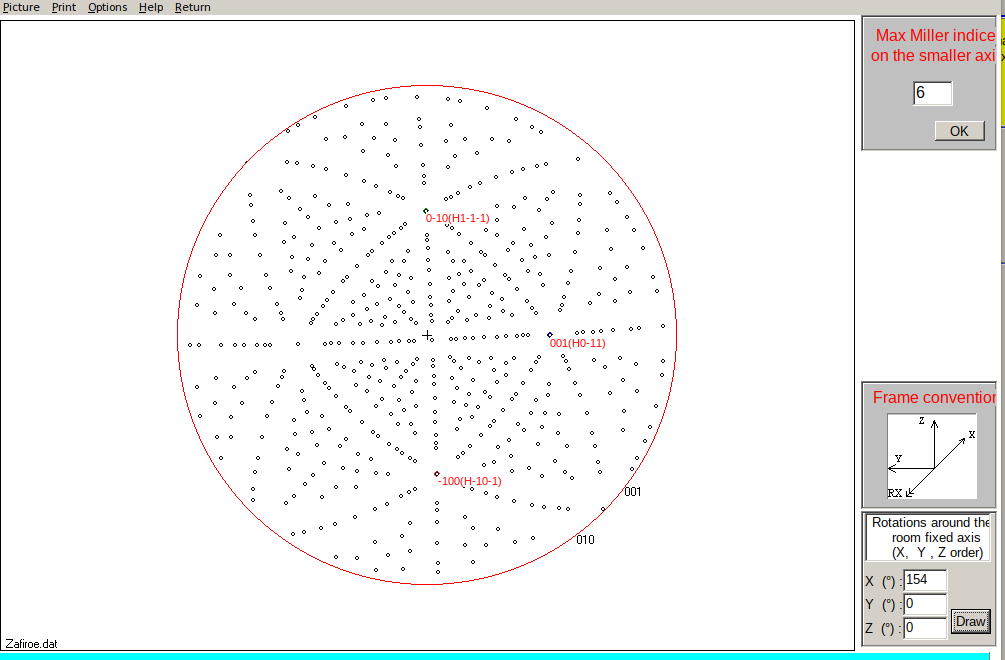
\includegraphics[width=0.6\textwidth]{./valid_indexation/Zafir-stereo.png}
	\caption{Stereo}
\end{figure}

\section{ Összegzés}

\par Itt is, mint általánosságban elmondható, hogy nem túlzottan sok, az életben
hasznosítható tudást halmoztunk fel a labor teljesítésével, azonban rengeteg időt
elpazarolhattunk egy nem működő szoftver használatával.

\end{document}